% Provenance (never printed): see sources/outline_sources.md (Year 1: rigid plates on a
% sphere, Euler poles and angular velocities; relative velocities; triple junctions;
% finite rotations; the magnetic-anomaly timescale; satellite geodesy). Curves and maps
% from figdata/bachelor-1/euler_velocities.py, south_atlantic_fit.py and gpts_stripes.py;
% exercise and problem values in the Book 3 scratch calculator calc/ch12.py.
\chapter{Plate Kinematics on a Sphere}\label{ch:b1:plate-kinematics}

Two satellite-positioning stations have been recording their positions every
day for more than a quarter of a century: one in Reykjavik, in the west of
Iceland, the other near Stavanger, on the west coast of Norway. The straight
line between them, \qty{1546}{km} long, grows by \qty{17.5}{mm} every year,
nearly two centimetres. Nothing on the ground shows it, yet the floor of the
North Atlantic between the two stations records the same widening over millions
of years: lava erupted at the Mid-Atlantic Ridge took on the direction of the
Earth's magnetic field as it cooled, and the field has reversed many times, so
that the ocean floor carries a striped record of its own growth. This chapter
turns the plates of the school years into rigid caps on a sphere, describes
their motions with the geometry of rotations, and shows how the geological
record and the satellites measure the same motions.
% ledger: ngl:reyk, ngl:stas (chord lengthening computed in calc/ch12.py)

\begin{recall}
On a sphere, a \omterm{def:b1:spherical-astronomy:spherical-triangle}{great circle} is the intersection with a plane through the
centre, a \omterm{def:b1:spherical-astronomy:spherical-triangle}{small circle} with any other plane; the cosine rule gives the angular
distance between two points from their \omterm{def:b1:spherical-astronomy:geographic}{latitudes} and \omterm{def:b1:spherical-astronomy:geographic}{longitudes}, and the
\omterm{def:b1:spherical-astronomy:horizontal}{azimuth} of a direction is counted from north through east
(\cref{ch:b1:spherical-astronomy}). A rigid body turning about a fixed axis has
an angular velocity (physics). The \omterm{def:b1:layered-earth:lithosphere}{lithosphere} is broken into plates that move
relative to one another at a few centimetres a year, and the ocean floor
carries magnetic stripes that record the reversals of the Earth's magnetic
field (Book 2, grade 11).
\end{recall}

\section{Rigid plates on a sphere}

A plate covers a large part of the sphere: the Eurasian plate stretches from
the middle of the Atlantic to eastern Siberia. Its motion cannot be described by a velocity, as the
motion of a car can; it must be described by a rotation.

\begin{definition}[Rigid plate]\label{def:b1:plate-kinematics:rigid-plate}
A \emph{rigid plate}\index{rigid plate} is a region of the \omterm{def:b1:layered-earth:lithosphere}{lithosphere} whose
interior does not deform measurably: the distance between any two of its points
stays constant. The relative motion of two plates is taken up along their
common boundary, a narrow zone of faults, earthquakes and volcanoes.
\end{definition}

No plate is perfectly rigid: the boundaries are zones tens to hundreds of
kilometres wide, and the interiors deform slowly. The hypothesis is that these
departures are small beside the relative motions; it is tested by the
consistency of every result of this chapter.

A \omterm{def:b1:plate-kinematics:rigid-plate}{rigid plate} on the surface of a sphere moves without changing the distance
between any two of its points, and the centre of the Earth does not move. Such
a motion is described by a $3\times3$ matrix $R$ that keeps lengths, an
\emph{orthogonal} matrix ($R^{\mathsf T}R = I$), and that keeps the orientation
of space, so that $\det R = 1$: a point at the position vector $\vec r$ goes to
$R\vec r$.

\begin{theorem}[Euler's rotation theorem]\label{thm:b1:plate-kinematics:euler}
Every displacement of a \omterm{def:b1:plate-kinematics:rigid-plate}{rigid plate} on the sphere is a rotation about an axis
through the centre of the Earth: there is a unit vector $\vec n$ with
$R\vec n = \vec n$, and the plate turns about $\vec n$ by some angle.
\end{theorem}

\begin{proof}
We show that $1$ is an eigenvalue of $R$, that is $\det(R - I) = 0$. Since
$R R^{\mathsf T} = I$, we have $R - I = R(I - R^{\mathsf T})$, so
\[
  \det(R - I) = \det R\,\det\bigl((I - R)^{\mathsf T}\bigr) = \det(I - R),
\]
using $\det R = 1$ and the fact that a matrix and its transpose have the same
determinant. For a $3\times3$ matrix,
$\det(I - R) = (-1)^3\det(R - I) = -\det(R - I)$. So $\det(R - I) =
-\det(R - I)$, which is zero. A unit vector $\vec n$ with $R\vec n = \vec n$
therefore exists: the two points where the line through the centre along
$\vec n$ meets the surface do not move. In the plane perpendicular to $\vec n$,
$R$ keeps lengths and orientation: it turns that plane by some angle, and so
it turns the whole sphere about $\vec n$.
\end{proof}

Over an interval of time short enough for the motion not to change, the
rotation proceeds at a steady rate, and the motion of one plate relative to
another is an angular velocity about a fixed axis.

\begin{definition}[Euler pole; Euler vector]\label{def:b1:plate-kinematics:euler-pole}
The motion of a plate B relative to a plate A is a rotation about an axis
through the centre of the Earth. The \emph{Euler pole}\index{Euler pole} of the
pair is the point where this axis meets the surface, chosen so that the
rotation is anticlockwise seen from above it; the antipodal point is the
opposite pole. The \emph{Euler vector}\index{Euler vector}
$\vec\omega_{BA}$ is the angular velocity of B relative to A: it points from
the centre of the Earth towards the Euler pole, and its length $\omega$ is the
rate of rotation.
\end{definition}

An \omterm{def:b1:plate-kinematics:euler-pole}{Euler vector} is given by the \omterm{def:b1:spherical-astronomy:geographic}{latitude} and \omterm{def:b1:spherical-astronomy:geographic}{longitude} of its pole and its
rate, usually in degrees per million years. The motion of the Eurasian plate
relative to the North American plate, averaged over the last \qty{3.16}{Myr}
from 453 spreading rates measured on the ridges between them, has its pole at
\ang{61.8}\,N, \ang{139.6}\,E, in eastern Siberia, and the rate
\qty{0.210}{\degree\per\Myr}. In radians per year,
\[
  \omega = \frac{0.210\times\pi/180}{\num{e6}} = \qty{3.665e-9}{rad.yr^{-1}},
\]
a full turn in \qty{1714}{\Myr}.
% ledger: morvel:eu-na, morvel:summary

\section{Relative velocities}

\begin{theorem}[Velocity on a rotating plate]\label{thm:b1:plate-kinematics:velocity}
If plate B turns relative to plate A with the \omterm{def:b1:plate-kinematics:euler-pole}{Euler vector} $\vec\omega$, a point
of B at the position vector $\vec r$ (from the centre of the Earth) moves
relative to A with the velocity
\[
  \vec v = \vec\omega\times\vec r .
\]
\end{theorem}

\begin{proof}
Let $\Delta$ be the angle between $\vec\omega$ and $\vec r$. As B turns, the
point describes a circle about the axis, of radius $R\sin\Delta$, where $R$ is
the radius of the Earth; at the angular rate $\omega$, its speed is
$\omega R\sin\Delta$. Its velocity is tangent to that circle, so perpendicular
both to the axis and to the radius $\vec r$, and the rotation being
anticlockwise about $\vec\omega$, its sense is that of $\vec\omega\times\vec r$.
The vector $\vec\omega\times\vec r$ has precisely this direction and sense and
the length $\omega R\sin\Delta$.
\end{proof}

The angle $\Delta$ is the angular distance between the \omterm{def:b1:plate-kinematics:euler-pole}{Euler pole} and the point,
which the cosine rule gives from \omterm{def:b1:spherical-astronomy:geographic}{latitudes} and \omterm{def:b1:spherical-astronomy:geographic}{longitudes}.

\begin{proposition}[Speed and direction of relative motion]\label{prop:b1:plate-kinematics:speed}
Let the \omterm{def:b1:plate-kinematics:euler-pole}{Euler pole} be at \omterm{def:b1:spherical-astronomy:geographic}{latitude} $\varphi_p$ and \omterm{def:b1:spherical-astronomy:geographic}{longitude} $\lambda_p$, and the
point at $\varphi$ and $\lambda$. Then
\begin{enumerate}
  \item the angular distance $\Delta$ from the pole to the point satisfies
        $\cos\Delta = \sin\varphi_p\sin\varphi + \cos\varphi_p\cos\varphi
        \cos(\lambda - \lambda_p)$;
  \item the relative speed is $v = \omega R\sin\Delta$: zero at the pole,
        largest, $\omega R$, on the \omterm{def:b1:spherical-astronomy:spherical-triangle}{great circle} \ang{90} from it;
  \item the direction of motion is perpendicular to the \omterm{def:b1:spherical-astronomy:spherical-triangle}{great circle} that joins
        the point to the pole: its \omterm{def:b1:spherical-astronomy:horizontal}{azimuth} is that of the pole, as seen from
        the point, plus \ang{90}.
\end{enumerate}
\end{proposition}

\begin{proof}
(1) is the cosine rule in the \omterm{def:b1:spherical-astronomy:spherical-triangle}{spherical triangle} formed by the geographic north
pole, the \omterm{def:b1:plate-kinematics:euler-pole}{Euler pole} and the point, whose sides from the north pole are
$\ang{90} - \varphi_p$ and $\ang{90} - \varphi$, with the angle
$\lambda - \lambda_p$ between them. (2) follows from the theorem. (3) The
velocity is perpendicular to $\vec\omega$ and to $\vec r$, so to the plane that
contains them, the plane of the \omterm{def:b1:spherical-astronomy:spherical-triangle}{great circle} through the point and the pole. In
the horizontal plane at the point, it is therefore perpendicular to the
direction of the pole; the rotation being anticlockwise seen from above the
pole, a point moves to the right of the direction in which it sees the pole,
which adds \ang{90} to the \omterm{def:b1:spherical-astronomy:horizontal}{azimuth}.
\end{proof}

\begin{omfigure}
\begin{tikzpicture}[x=2.5cm, y=2.5cm, font=\scriptsize, >=Stealth]
% orthographic view from 20 deg above the "Euler equator": a point at polar angle D,
% longitude p about the pole projects to X = sin D sin p, Y = cos D cos 20 - sin D cos p sin 20;
% it is visible when cos p >= -cot D tan 20 (limits computed by hand: 129.08, 102.13, 90, 77.87)
\fill[omSea!12] (0,0) circle (1);
\draw[thick] (0,0) circle (1);
\foreach \D/\m in {30/129.08, 60/102.13, 90/90, 120/77.87} {
  \draw[blue!45!black, domain=-\m:\m, samples=60, variable=\p]
    plot ({sin(\D)*sin(\p)}, {cos(\D)*cos(20) - sin(\D)*cos(\p)*sin(20)});
  \draw[blue!45!black, densely dashed, domain=\m:360-\m, samples=60, variable=\p]
    plot ({sin(\D)*sin(\p)}, {cos(\D)*cos(20) - sin(\D)*cos(\p)*sin(20)});
}
\draw[densely dashed] (0,0) -- (0,0.9397);
\draw[->, very thick] (0,0.9397) -- (0,1.38) node[above] {$\vec\omega$};
\fill (0,0.9397) circle (0.9pt) node[anchor=south west] {Euler pole};
\fill (0,0) circle (0.7pt);
% velocity arrows at longitude -35 deg about the pole, length 0.5 sin D
\draw[->, very thick, red!75!black] (-0.287,0.6737) -- ++(0.243,-0.058);
\draw[->, very thick, red!75!black] (-0.497,0.2272) -- ++(0.421,-0.101);
\draw[->, very thick, red!75!black] (-0.574,-0.2802) -- ++(0.487,-0.117);
\draw[->, very thick, red!75!black] (-0.497,-0.7124) -- ++(0.421,-0.101);
\draw[->] (0,0) -- (-0.497,0.2272) node[pos=0.55, below] {$\vec r$};
\draw (0,0.22) arc[start angle=90, end angle=155.4, radius=0.22];
\node at (-0.11,0.33) {$\Delta$};
\node[anchor=west] at (0.62,0.81) {$\Delta = \ang{30}$};
\node[anchor=west] at (0.88,0.47) {$\Delta = \ang{60}$};
\node[anchor=west] at (1.02,0.0) {$\Delta = \ang{90}$};
\node[anchor=west] at (0.88,-0.47) {$\Delta = \ang{120}$};
\end{tikzpicture}

\par\smallskip{\small A plate turning about its \omterm{def:b1:plate-kinematics:euler-pole}{Euler pole}, seen from a little
above the circle \ang{90} from the pole. Every point moves along a \omterm{def:b1:spherical-astronomy:spherical-triangle}{small circle}
about the pole (hidden parts dashed); its speed, shown by the red arrows, is
$\omega R\sin\Delta$, where $\Delta$ is its angular distance from the pole: zero
at the pole, largest \ang{90} away.}
\label{fig:b1:plate-kinematics:euler-pole}
\end{omfigure}

The speed of relative motion therefore changes along a plate boundary even
when the two plates are perfectly rigid, and the direction of motion turns with
it. Two consequences shape every plate boundary map.

\begin{proposition}[Transforms follow small circles]\label{prop:b1:plate-kinematics:transforms}
A transform fault, along which two plates slide past each other without
opening or closing, lies on a \omterm{def:b1:spherical-astronomy:spherical-triangle}{small circle} about the \omterm{def:b1:plate-kinematics:euler-pole}{Euler pole} of the two
plates. The direction of spreading at a ridge, and of convergence at a
subduction zone, is along the \omterm{def:b1:spherical-astronomy:spherical-triangle}{small circles} too.
\end{proposition}

\begin{proof}
On a transform fault the relative velocity is parallel to the fault at every
point. The relative velocity is everywhere tangent to the \omterm{def:b1:spherical-astronomy:spherical-triangle}{small circles} about
the pole (\cref{thm:b1:plate-kinematics:velocity}); a curve tangent at each of
its points to the \omterm{def:b1:spherical-astronomy:spherical-triangle}{small circle} through that point is one of these circles. The
second statement is the third part of \cref{prop:b1:plate-kinematics:speed}.
\end{proof}

The Mid-Atlantic Ridge between Eurasia and North America is a staircase of
ridge segments offset by transform faults; the transforms \omterm{def:b1:field-lab-methods-1:trend-plunge}{trend} close to the
\omterm{def:b1:spherical-astronomy:horizontal}{azimuths} the \omterm{def:b1:plate-kinematics:euler-pole}{Euler vector} predicts, and their \omterm{def:b1:field-lab-methods-1:trend-plunge}{trend} is one of the data used to
locate the pole. The spreading rate along the same boundary grows with the
angular distance from the pole: \qtyrange{11}{12}{mm.yr^{-1}} on the Gakkel
Ridge in the Arctic Ocean, near the pole, and \qty{23}{mm.yr^{-1}} just north
of the Azores, \ang{78} from it. The figure below compares the rates the \omterm{def:b1:plate-kinematics:euler-pole}{Euler
vector} predicts all along the boundary with those of an independent plate model.
% ledger: morvel:eu-na

\begin{method}[The velocity at a point]\label{met:b1:plate-kinematics:velocity}
\begin{enumerate}
  \item Convert the rate of the \omterm{def:b1:plate-kinematics:euler-pole}{Euler vector} to radians per year and compute
        $\omega R$, in \unit{mm.yr^{-1}} with $R = \qty{6371}{km}$.
  \item Compute the angular distance $\Delta$ from the pole to the point with
        the cosine rule; the speed is $\omega R\sin\Delta$.
  \item Compute the \omterm{def:b1:spherical-astronomy:horizontal}{azimuth} $\beta$ of the pole as seen from the point, with
        $\tan\beta = \sin(\lambda_p - \lambda)\cos\varphi_p /
        \bigl(\cos\varphi\sin\varphi_p - \sin\varphi\cos\varphi_p
        \cos(\lambda_p - \lambda)\bigr)$ and the quadrant of the numerator and
        denominator; the motion is towards $\beta + \ang{90}$.
  \item Check the sense: the motion is the one of the second plate relative to
        the first. Exchanging the plates reverses it.
\end{enumerate}
\end{method}

\begin{example}[Eurasia moves away from North America in Iceland]\label{ex:b1:plate-kinematics:iceland}
Take the middle of Iceland at \ang{64.5}\,N, \ang{18}\,W, and the \omterm{def:b1:plate-kinematics:euler-pole}{Euler vector}
of Eurasia relative to North America above. Then $\omega R =
\num{3.665e-9}\times\qty{6.371e9}{mm} = \qty{23.35}{mm.yr^{-1}}$, and
\[
  \cos\Delta = \sin\ang{61.8}\sin\ang{64.5}
  + \cos\ang{61.8}\cos\ang{64.5}\cos(\ang{-18} - \ang{139.6}) = 0.60736,
\]
so $\Delta = \ang{52.60}$ and $v = 23.35\sin\ang{52.60} = \qty{18.55}{mm.yr^{-1}}$.
The pole is seen at the \omterm{def:b1:spherical-astronomy:horizontal}{azimuth} $\beta = \ang{13.1}$, a little east of north,
over the Arctic; Eurasia moves towards $\ang{103.1}$, east-south-east, that is
\qty{18.07}{mm.yr^{-1}} to the east and \qty{4.20}{mm.yr^{-1}} to the south.
% computed in calc/ch12.py and figdata/bachelor-1/euler_velocities.py
\end{example}

\begin{omfigure}
\begin{tikzpicture}
\begin{axis}[omrecord, width=0.84\linewidth, height=6.4cm, xmin=0, xmax=90, ymin=0, ymax=26,
  xtick={0,15,...,90}, xlabel={angular distance from the Euler pole, $\Delta$ (degrees)},
  ylabel={spreading rate (\unit{mm.yr^{-1}})},
  legend style={font=\scriptsize, at={(0.99,0.03)}, anchor=south east, draw=none, fill=white, fill opacity=0.85, text opacity=1},
  legend cell align=left]
% computed in figdata/bachelor-1/euler_velocities.py
\addplot[only marks, mark=*, mark size=0.9pt, black!55] table[x=delta, y=pb2002] {figdata/out/bachelor-1-euler_velocities-mar.dat};
\addlegendentry{plate boundary model PB2002, every boundary step}
\addplot[only marks, mark=x, mark size=1.1pt, blue!60!black] table[x=delta, y=gps] {figdata/out/bachelor-1-euler_velocities-mar.dat};
\addlegendentry{Euler vector from satellite positioning}
\addplot[very thick, red!75!black] table[x=delta, y=v] {figdata/out/bachelor-1-euler_velocities-curve.dat};
\addlegendentry{$\omega R\sin\Delta$, geological Euler vector}
\node[font=\scriptsize, anchor=south east] at (axis cs:52.6,19.6) {Iceland};
\draw[black!70] (axis cs:52.6,18.55) circle (2.5pt);
\node[font=\scriptsize, anchor=south] at (axis cs:78.4,23.6) {Azores};
\draw[black!70] (axis cs:78.4,22.87) circle (2.5pt);
\node[font=\scriptsize, anchor=south] (gk) at (axis cs:9,12) {Gakkel Ridge};
\draw[black!70, -{Stealth[length=3pt]}] (gk.south) -- (axis cs:16.5,7.2);
\end{axis}
\end{tikzpicture}

\par\smallskip{\small Spreading rates between Eurasia and North America, from
the Arctic Ocean to the Azores, against the angular distance from the \omterm{def:b1:plate-kinematics:euler-pole}{Euler
pole}. Red: the geological \omterm{def:b1:plate-kinematics:euler-pole}{Euler vector} (pole \ang{61.8}\,N, \ang{139.6}\,E,
\qty{0.210}{\degree\per\Myr}), which puts all the rates on one sine curve. Grey:
the rates of an independent plate boundary model at each of its boundary steps;
they differ from the curve by \qty{1}{\percent} on average. Blue: the rates
predicted at the same steps by an \omterm{def:b1:plate-kinematics:euler-pole}{Euler vector} computed from satellite
positioning in the two plate interiors (pole \ang{74.2}\,N, \ang{134.1}\,E,
\qty{0.237}{\degree\per\Myr}): its pole being elsewhere, its rates do not lie on
the red curve. They are within a tenth of the geological rates from the Azores
to Iceland, and much lower in the Arctic, where the rates are small and depend
strongly on the exact position of the pole.}
\label{fig:b1:plate-kinematics:mar-rates}
\end{omfigure}
% ledger: morvel:eu-na, morvel:gps-eu-na, data:pb2002 (mean difference 0.96 per cent, euler_velocities.py)

\section{Combining motions; triple junctions}

Relative velocities add like the velocities of mechanics: if B moves relative to
A and C relative to B, then C moves relative to A with the sum of the two
velocities.

\begin{proposition}[Euler vectors add]\label{prop:b1:plate-kinematics:addition}
For three plates A, B, C,
\[
  \vec\omega_{CA} = \vec\omega_{CB} + \vec\omega_{BA}, \qquad
  \vec\omega_{AB} = -\vec\omega_{BA}.
\]
\end{proposition}

\begin{proof}
At every point $\vec r$, $\vec v_{CA} = \vec v_{CB} + \vec v_{BA}$, that is
$\vec\omega_{CA}\times\vec r = \vec\omega_{CB}\times\vec r +
\vec\omega_{BA}\times\vec r = (\vec\omega_{CB} + \vec\omega_{BA})\times\vec r$
by the linearity of the cross product. A vector $\vec u$ with
$\vec u\times\vec r = \vec 0$ for every $\vec r$ is zero, so the two \omterm{def:b1:plate-kinematics:euler-pole}{Euler
vectors} are equal. Exchanging A and B reverses every velocity.
\end{proof}

To add \omterm{def:b1:plate-kinematics:euler-pole}{Euler vectors}, write each in Cartesian components, $\omega(\cos\varphi_p
\cos\lambda_p, \cos\varphi_p\sin\lambda_p, \sin\varphi_p)$, add the components,
and convert back to a pole and a rate. Poles cannot be added; \omterm{def:b1:plate-kinematics:euler-pole}{Euler vectors}
can. The relation is a powerful constraint. The motion of the Nubian plate
(Africa) relative to Eurasia is slow, and the geological record gives few
direct measures of it: between the Azores and Gibraltar, the only ones are the
\omterm{def:b1:spherical-astronomy:horizontal}{azimuths} of a single transform, the Gloria fault. It follows instead from the
two well-measured spreading motions across the Atlantic: with $\vec\omega_{\mathrm{NB\,NA}}$ (pole
\ang{79.2}\,N, \ang{40.2}\,E, \qty{0.233}{\degree\per\Myr}) and
$\vec\omega_{\mathrm{EU\,NA}}$ above, $\vec\omega_{\mathrm{NB\,EU}} =
\vec\omega_{\mathrm{NB\,NA}} - \vec\omega_{\mathrm{EU\,NA}}$ has its pole at
\ang{20.9}\,N, \ang{18.3}\,W, off West Africa, and the rate
\qty{0.123}{\degree\per\Myr} (\cref{exo:b1:plate-kinematics:7}).
% ledger: morvel:nb-na, morvel:eu-na, morvel:nb-eu

\begin{definition}[Triple junction; stable triple junction]\label{def:b1:plate-kinematics:triple-junction}
A \emph{triple junction}\index{triple junction} is a point where three plates
meet, and with them three plate boundaries, each a ridge (R), a trench (T) or a
transform fault (F). A triple junction is \emph{stable}\index{stable triple
junction} if, as the plates move, it keeps the same geometry: the same three
kinds of boundary meeting at the same angles.
\end{definition}

Each boundary allows the junction to move only in certain ways without changing
its geometry. A symmetric ridge stays midway between its two plates; a
transform keeps its \omterm{def:b1:field-lab-methods-1:trend-plunge}{trend} whatever the junction does along it; a trench is
fixed to its overriding plate. The question is whether one motion of the
junction satisfies all three boundaries at once. It is answered in
\emph{velocity space}: a diagram in which each plate is a point whose position
vector is the plate's velocity at the junction, relative to any one plate, so
that the side joining two points is the relative velocity of the two plates.

\begin{proposition}[Ridge--ridge--ridge junctions are stable]\label{prop:b1:plate-kinematics:rrr}
A junction of three ridges, each spreading symmetrically and perpendicular to
its axis, is \omterm{def:b1:plate-kinematics:triple-junction}{stable} whatever the relative velocities of the three plates.
\end{proposition}

\begin{proof}
Let $a$, $b$, $c$ be the points of the three plates in velocity space. A ridge
between A and B that spreads symmetrically moves at the mean velocity of its
two plates, $(a + b)/2$, plus any velocity along its own axis, which is
perpendicular to $ab$: the velocities of the junction that leave the ridge
unchanged form the perpendicular bisector of the side $ab$. The junction keeps
its geometry if its velocity lies on the three perpendicular bisectors at once.
The three perpendicular bisectors of a triangle always meet at one point, the
centre of its circumscribed circle. So a velocity of the junction always
exists.
\end{proof}

McKenzie and Morgan, who introduced the distinction between \omterm{def:b1:plate-kinematics:triple-junction}{stable} and unstable
junctions in 1969, analysed the combinations in this way. A transform allows the
junction to move only along itself, that is, along the line through the points
of its two plates: a junction of three transforms is therefore never \omterm{def:b1:plate-kinematics:triple-junction}{stable},
since the three lines through the sides of a triangle have no common point. For
the other kinds, stability places conditions on the orientations of the
boundaries and on the relative velocities.
% ledger: mckenzie:triple-junctions

\begin{omfigure}
\begin{tikzpicture}[font=\scriptsize, >=Stealth]
% (a) map view of an RRR junction, ridges perpendicular to the sides of the
% velocity triangle in (b): ray directions 110.6, -121.0, -10.8 degrees
\begin{scope}[x=1cm, y=1cm]
  \node[font=\small] at (0,2.25) {(a) map};
  \fill[omSea!12] (-2.4,-2.0) rectangle (2.4,2.0);
  \draw[ridge] (0,0) -- (110.6:2.0);
  \draw[ridge] (0,0) -- (-121.0:2.1);
  \draw[ridge] (0,0) -- (-10.8:2.3);
  \fill (0,0) circle (1.5pt) node[anchor=south west] {J};
  \node[font=\normalsize] at (-1.5,0.3) {A};
  \node[font=\normalsize] at (1.4,1.1) {B};
  \node[font=\normalsize] at (0.7,-1.4) {C};
  \draw[->, thick] ($(110.6:1.3)+(20.6:0.12)$) -- ++(20.6:0.45);
  \draw[->, thick] ($(110.6:1.3)+(200.6:0.12)$) -- ++(200.6:0.45);
  \draw[->, thick] ($(-121:1.3)+(-31:0.12)$) -- ++(-31:0.45);
  \draw[->, thick] ($(-121:1.3)+(149:0.12)$) -- ++(149:0.45);
  \draw[->, thick] ($(-10.8:1.5)+(-100.8:0.12)$) -- ++(-100.8:0.45);
  \draw[->, thick] ($(-10.8:1.5)+(79.2:0.12)$) -- ++(79.2:0.45);
\end{scope}
% (b) velocity space: a(0,0), b(2.4,0.9), c(2.0,-1.2); circumcentre (1.365, 0.009)
\begin{scope}[xshift=5.6cm, yshift=-0.2cm, x=1.25cm, y=1.25cm]
  \node[font=\small] at (1.2,1.95) {(b) velocity space};
  \draw[thick] (0,0) -- (2.4,0.9) -- (2.0,-1.2) -- cycle;
  \fill (0,0) circle (1.5pt) node[left] {$a$};
  \fill (2.4,0.9) circle (1.5pt) node[above right] {$b$};
  \fill (2.0,-1.2) circle (1.5pt) node[below right] {$c$};
  \draw[omRidge!80!black, densely dashed] ($(1.365,0.009)+(-0.351*1.4,0.936*1.4)$) -- ($(1.365,0.009)+(0.351*0.9,-0.936*0.9)$);
  \draw[omRidge!80!black, densely dashed] ($(1.365,0.009)+(0.982*1.5,-0.187*1.5)$) -- ($(1.365,0.009)+(-0.982*0.6,0.187*0.6)$);
  \draw[omRidge!80!black, densely dashed] ($(1.365,0.009)+(-0.514*1.6,-0.857*1.6)$) -- ($(1.365,0.009)+(0.514*0.6,0.857*0.6)$);
  \fill[omRidge!80!black] (1.365,0.009) circle (1.6pt);
  \node[anchor=north, omRidge!80!black] at (1.30,-0.05) {$j$};
  \node[anchor=south east] at (1.05,0.50) {$ab$};
\end{scope}
\end{tikzpicture}

\par\smallskip{\small A junction J of three ridges between plates A, B and C.
(a) Map: each ridge (double line) spreads perpendicular to its axis (arrows).
(b) Velocity space: each plate is a point; the side $ab$ is the velocity of B
relative to A, perpendicular to the ridge between them. The velocities of the
junction that leave a symmetric ridge unchanged form the perpendicular bisector
of the corresponding side (dashed); the three bisectors always meet, at $j$,
the velocity of the junction.}
\label{fig:b1:plate-kinematics:rrr}
\end{omfigure}

The Azores \omterm{def:b1:plate-kinematics:triple-junction}{triple junction}, at about \ang{39.4}\,N, \ang{29.8}\,W, where the
North American, Eurasian and Nubian plates meet, is a ridge--ridge--ridge
junction: the Mid-Atlantic Ridge runs north and south of it, and the slow
Terceira Rift runs east-south-east from it. At the junction the two \omterm{def:b1:plate-kinematics:euler-pole}{Euler
vectors} of the North American pair give Eurasia \qty{22.9}{mm.yr^{-1}} towards
\ang{95} and Nubia \qty{19.2}{mm.yr^{-1}} towards \ang{104}; Eurasia therefore
moves away from Nubia at \qty{4.9}{mm.yr^{-1}} towards \ang{59}, an
east-north-east--west-south-west opening across the Terceira rift. The real
junction is not a point: the spreading rate along the ridge falls gradually
from \qty{22.9}{mm.yr^{-1}} at \ang{40}\,N to \qty{19.8}{mm.yr^{-1}} at
\ang{38}\,N, across a small plate about \qty{100}{km} wide caught between the
three large ones, the Azores microplate.
% ledger: morvel:azores, data:pb2002 (junction point at 39.40 N, 29.77 W, three spreading boundaries), morvel:nb-eu, morvel:eu-na, morvel:nb-na (velocities computed in calc/ch12.py)

\section{Finite rotations}

The \omterm{def:b1:plate-kinematics:euler-pole}{Euler vector} describes the motion now, averaged over a few million years.
To put the plates back where they were long ago, one needs the rotation that
carries a plate from its present position to its past one.

\begin{definition}[Finite rotation]\label{def:b1:plate-kinematics:finite-rotation}
A \emph{finite rotation}\index{finite rotation} is the rotation of the sphere,
given by a pole (\omterm{def:b1:spherical-astronomy:geographic}{latitude}, \omterm{def:b1:spherical-astronomy:geographic}{longitude}) and an angle, that carries a plate, or a
piece of its edge, from its present position to its position at a given time
relative to another plate. A positive angle turns anticlockwise seen from above
the pole.
\end{definition}

\begin{proposition}[Rodrigues' formula]\label{prop:b1:plate-kinematics:rodrigues}
The rotation by the angle $\alpha$ about the unit vector $\vec n$ carries the
vector $\vec r$ to
\[
  \vec r\,' = \cos\alpha\,\vec r + (1 - \cos\alpha)(\vec n\cdot\vec r)\,\vec n
  + \sin\alpha\,\vec n\times\vec r .
\]
\end{proposition}

\begin{proof}
Split $\vec r$ into its part along the axis, $\vec r_\parallel =
(\vec n\cdot\vec r)\vec n$, which the rotation does not change, and its part
perpendicular to it, $\vec r_\perp = \vec r - \vec r_\parallel$. The vector
$\vec n\times\vec r = \vec n\times\vec r_\perp$ has the length of $\vec r_\perp$,
is perpendicular to it and to $\vec n$, and is turned \ang{90} anticlockwise from
it about $\vec n$. In the plane perpendicular to $\vec n$, the rotation by
$\alpha$ carries $\vec r_\perp$ to $\cos\alpha\,\vec r_\perp +
\sin\alpha\,\vec n\times\vec r$. Adding $\vec r_\parallel$ gives $\vec r\,' =
\vec r_\parallel + \cos\alpha(\vec r - \vec r_\parallel) + \sin\alpha\,
\vec n\times\vec r$, which is the formula.
\end{proof}

The formula is linear in $\vec r$; written with matrices, $\vec r\,' = R\vec r$
with
\[
  R = \cos\alpha\,I + (1 - \cos\alpha)\,\vec n\,\vec n^{\mathsf T}
  + \sin\alpha
  \begin{pmatrix} 0 & -n_z & n_y\\ n_z & 0 & -n_x\\ -n_y & n_x & 0\end{pmatrix},
\]
an orthogonal matrix of determinant $1$, as Euler's theorem requires. Its trace
is $1 + 2\cos\alpha$, which gives the angle of any rotation matrix
(\cref{exo:b1:plate-kinematics:10}).

\omterm{def:b1:plate-kinematics:finite-rotation}{Finite rotations} do not commute. Turn the point at \ang{0}\,N, \ang{0}\,E, on
the $x$ axis, by \ang{90} about the north pole: it goes to \ang{0}\,N,
\ang{90}\,E, on the $y$ axis; then by \ang{90} about the $x$ axis: it reaches
the north pole. Done in the other order, the first rotation leaves the point
where it is and the second takes it to \ang{0}\,N, \ang{90}\,E (\cref{exo:b1:plate-kinematics:8}).
A succession of plate motions must therefore be composed by multiplying the
matrices in the right order, never by adding angles; only angular velocities,
which describe infinitely small rotations, add as vectors.

\begin{omfigure}
\begin{tikzpicture}
\begin{axis}[axis equal image, width=0.8\linewidth, xmin=-85, xmax=55, ymin=-58, ymax=38,
  xtick={-80,-60,...,40}, ytick={-40,-20,0,20},
  xticklabel={$\pgfmathprintnumber{\tick}^\circ$}, yticklabel={$\pgfmathprintnumber{\tick}^\circ$},
  tick label style={font=\scriptsize}, axis background/.style={fill=omSea!10},
  unbounded coords=jump]
% computed in figdata/bachelor-1/south_atlantic_fit.py
\addplot[fill=omHypsLandC!60, draw=black!60, line width=0.3pt] table[x=lon, y=lat] {figdata/out/bachelor-1-south_atlantic_fit-af.dat};
\addplot[draw=black, line width=0.5pt] table[x=lon, y=lat] {figdata/out/bachelor-1-south_atlantic_fit-sa.dat};
\addplot[draw=blue!60!black, densely dashed, line width=0.6pt] table[x=lon, y=lat] {figdata/out/bachelor-1-south_atlantic_fit-sa84.dat};
\addplot[fill=red!40, fill opacity=0.55, draw=red!70!black, line width=0.5pt] table[x=lon, y=lat] {figdata/out/bachelor-1-south_atlantic_fit-sa120.dat};
\addplot[red!70!black, thick, densely dotted, -{Stealth}] table[x=lon, y=lat] {figdata/out/bachelor-1-south_atlantic_fit-track.dat};
\fill (axis cs:-34.9,-8.05) circle (1.6pt);
\node[font=\scriptsize, anchor=south east, fill=white, fill opacity=0.8, text opacity=1, inner sep=1pt] at (axis cs:-36,-7) {Recife};
\node[font=\scriptsize, align=center] at (axis cs:-60,-17) {South America\\today};
\node[font=\scriptsize, blue!60!black, anchor=east] at (axis cs:-31,-46) {83.5 Ma};
\node[font=\scriptsize, red!60!black, fill=white, fill opacity=0.8, text opacity=1, inner sep=1pt] at (axis cs:-8,-22) {120.6 Ma};
\node[font=\scriptsize] at (axis cs:22,12) {Africa};
\end{axis}
\end{tikzpicture}

\par\smallskip{\small Closing the South Atlantic. South America (black outline)
is carried back relative to Africa by two published \omterm{def:b1:plate-kinematics:finite-rotation}{finite rotations}: to its
position at \qty{83.5}{Ma} (pole \ang{61.88}\,N, \ang{34.26}\,W, angle
\ang{33.51}; dashed) and at \qty{120.6}{Ma}, as the ocean began to open (pole
\ang{51.28}\,N, \ang{33.67}\,W, angle \ang{52.35}; red). The dotted line is the
path of Recife on its \omterm{def:b1:spherical-astronomy:spherical-triangle}{small circle} about the older pole. \omterm{def:b1:spherical-astronomy:geographic}{Latitude} and \omterm{def:b1:spherical-astronomy:geographic}{longitude}
are drawn as a square grid, which stretches shapes away from the equator.
Coastlines: Natural Earth.}
\label{fig:b1:plate-kinematics:south-atlantic}
\end{omfigure}
% ledger: heine:sam-saf, data:ne-land

The fit of the coasts of South America and Africa, long noticed on maps,
becomes a calculation. With the rotation of
\qty{120.6}{Ma}, the coast of north-east Brazil near Recife (\ang{8.05}\,S,
\ang{34.9}\,W) lands at \ang{3.4}\,N, \ang{8.3}\,E, on the coast of the Gulf of
Guinea, after a journey of about \qty{5000}{km} along its \omterm{def:b1:spherical-astronomy:spherical-triangle}{small circle}: an
average opening of some \qty{40}{mm.yr^{-1}}. The fit is not perfect
everywhere: for some fourteen million years before the ocean opened, the two
continents were slowly stretched apart, and a tight reconstruction must first
restore the stretched margins and rift basins on both sides.
% ledger: heine:sam-saf, heine:fit (Recife computed in south_atlantic_fit.py and calc/ch12.py)

\begin{history}[Tectonics on a sphere]
In 1965 Edward Bullard and two colleagues fitted the continents around the
Atlantic by computer, with a least-squares criterion: the best fit follows the
steep part of the continental edge, at a depth of 500 fathoms (about
\qty{900}{m}), not the coastline. The same year Tuzo Wilson described a new
class of faults, the transform faults, and their bearing on continental drift.
In 1967 Dan McKenzie and Robert Parker showed, with the North Pacific as their
example, that the aseismic areas of the surface move as \omterm{def:b1:plate-kinematics:rigid-plate}{rigid plates} on a
sphere. In 1968 Jason Morgan described the surface as crustal blocks bounded by
rises, trenches and great faults, and Xavier Le Pichon tied sea-floor spreading
to continental drift. Within three years, the drift of continents had become the
kinematics of rigid caps on a sphere.
% ledger: bullard:fit, wilson:transform, mckenzie:sphere, morgan:blocks, lepichon:spreading
\end{history}

\section{Measuring plate motions}

\subsection*{The magnetic record of the ocean floor}

Lava erupted at a ridge acquires, as it cools, a magnetization in the direction
of the Earth's field at that moment, and keeps it as it moves away from the
ridge. Since the field reverses at irregular intervals, the ocean floor is
magnetized in alternating directions, in bands parallel to the ridge.

\begin{definition}[Marine magnetic anomaly; polarity chron; polarity timescale]\label{def:b1:plate-kinematics:magnetic-anomaly}
A \emph{marine magnetic anomaly}\index{marine magnetic anomaly} is the
difference between the intensity of the magnetic field measured at sea and the
intensity of a reference model of the Earth's main field at the same place: it
is positive above \omterm{def:b1:layered-earth:layers}{crust} magnetized in the direction of the present field, and
negative above \omterm{def:b1:layered-earth:layers}{crust} magnetized in the opposite direction. A \emph{polarity
chron}\index{polarity chron} is an interval of time during which the field kept
one polarity, named by a number and the letter n (normal, as today) or r
(reversed). The \emph{geomagnetic polarity timescale}\index{geomagnetic
polarity timescale} is the sequence of polarity chrons with the ages of their
boundaries.
\end{definition}

The timescale is built by dating reversal sequences on land and in deep-sea
sediment cores, and by matching the pattern of the ocean-floor anomalies, whose
widths keep the relative durations of the chrons. The present normal chron, C1n, began
\qty{0.781}{Ma}, and the field has reversed at irregular intervals: the
timescale counts twenty-five normal intervals in the last eleven million years,
some lasting more than a million years, others little more than ten
thousand. The
figure below shows that history, down to the end of chron C5n, and the stripes
it writes on the floor of a slow and of a fast ridge.
% ledger: iodp:gpts2004

\begin{omfigure}
\begin{tikzpicture}
\begin{axis}[name=gpts, width=0.9\linewidth, height=2.3cm, xmin=0, xmax=11.04, ymin=0, ymax=1,
  ytick=\empty, xtick={0,1,...,11}, tick label style={font=\scriptsize}, axis on top,
  xlabel={age (Ma)}, label style={font=\scriptsize}, title={(a) polarity timescale, \qtyrange{0}{11}{Ma}},
  title style={font=\small, yshift=-1.5ex}]
% computed in figdata/bachelor-1/gpts_stripes.py
\addplot[const plot, fill=black, draw=none] table[x=age, y=pol] {figdata/out/bachelor-1-gpts_stripes-gpts.dat} \closedcycle;
\node[font=\scriptsize, fill=white, inner sep=1pt] at (axis cs:0.39,0.5) {C1n};
\node[font=\scriptsize, fill=white, inner sep=1pt] at (axis cs:3.1,0.5) {C2An};
\node[font=\scriptsize, fill=white, inner sep=1pt] at (axis cs:4.75,0.5) {C3n};
\node[font=\scriptsize, fill=white, inner sep=1pt] at (axis cs:10.42,0.5) {C5n};
\end{axis}
\begin{axis}[name=slow, at={(gpts.south west)}, anchor=north west, yshift=-1.75cm, width=0.9\linewidth,
  height=2.3cm, xmin=-110.4, xmax=110.4, ymin=0, ymax=1, ytick=\empty, xtick={-100,-50,0,50,100},
  tick label style={font=\scriptsize}, axis on top, xlabel={distance from the ridge axis (km)},
  label style={font=\scriptsize}, title={(b) half spreading rate \qty{10}{mm.yr^{-1}}},
  title style={font=\small, yshift=-1.5ex}]
\addplot[const plot, fill=black, draw=none] table[x=x, y=pol] {figdata/out/bachelor-1-gpts_stripes-stripes10.dat} \closedcycle;
\draw[red!80!black, very thick] (axis cs:0,0) -- (axis cs:0,1);
\end{axis}
\begin{axis}[at={(slow.south west)}, anchor=north west, yshift=-1.75cm, width=0.9\linewidth,
  height=2.3cm, xmin=-441.6, xmax=441.6, ymin=0, ymax=1, ytick=\empty, xtick={-400,-200,0,200,400},
  tick label style={font=\scriptsize}, axis on top, xlabel={distance from the ridge axis (km)},
  label style={font=\scriptsize}, title={(c) half spreading rate \qty{40}{mm.yr^{-1}}},
  title style={font=\small, yshift=-1.5ex}]
\addplot[const plot, fill=black, draw=none] table[x=x, y=pol] {figdata/out/bachelor-1-gpts_stripes-stripes40.dat} \closedcycle;
\draw[red!80!black, very thick] (axis cs:0,0) -- (axis cs:0,1);
\end{axis}
\end{tikzpicture}

\par\smallskip{\small (a) The \omterm{def:b1:plate-kinematics:magnetic-anomaly}{geomagnetic polarity timescale} over the last
\qty{11}{Myr} (black: normal polarity, as today; white: reversed), with the
ages of the 2004 timescale, short subchrons included. (b) and (c) The ocean
floor that a ridge (red) builds during the
same time, spreading symmetrically: every polarity interval becomes a pair of
stripes, one on each flank, of width equal to the \omterm{def:b1:plate-kinematics:spreading-rate}{half spreading rate} times its
duration. At four times the rate, the same pattern is four times wider; short
events such as the Jaramillo (near \qty{1}{Ma}) make stripes less than a
kilometre wide on the slow ridge.}
\label{fig:b1:plate-kinematics:stripes}
\end{omfigure}

\begin{definition}[Half and full spreading rates]\label{def:b1:plate-kinematics:spreading-rate}
At a ridge, the \emph{half spreading rate}\index{half spreading rate} of a
flank is the rate at which the \omterm{def:b1:layered-earth:layers}{crust} of that flank moves away from the ridge
axis. The \emph{full spreading rate}\index{full spreading rate} is the rate at
which the two plates move apart, the sum of the two half rates; it is twice the
half rate when the spreading is symmetric.
\end{definition}

\begin{method}[A spreading rate from magnetic anomalies]\label{met:b1:plate-kinematics:rate}
\begin{enumerate}
  \item On a magnetic profile perpendicular to the ridge, identify the sequence
        of anomalies on both flanks by its pattern of wide and narrow stripes,
        and match it to the polarity timescale.
  \item Measure the distance from the axis to the same chron boundary on each
        flank, and divide by its age: these are the two \omterm{def:b1:plate-kinematics:spreading-rate}{half spreading rates},
        averaged since that time. The full rate is their sum, or the distance
        between the two boundaries divided by the age.
  \item Prefer an old boundary to a young one: an error of a kilometre in a
        distance weighs less on a distance of a hundred kilometres than on one
        of ten.
  \item If the profile is not perpendicular to the ridge, project the distances
        onto the direction of spreading.
\end{enumerate}
\end{method}

The third point is not only a matter of reading errors. The \omterm{def:b1:layered-earth:layers}{crust} does not
acquire its magnetization along a single line: lava flows over the adjacent,
slightly older \omterm{def:b1:layered-earth:layers}{crust}, dykes intrude into it, and the lower \omterm{def:b1:layered-earth:layers}{crust} is magnetized
later than the upper. All these processes shift the boundaries between stripes
away from the axis, so that the distance between two boundaries of the same age
exceeds the width of \omterm{def:b1:layered-earth:layers}{crust} actually formed. The two-sided shift is
\qtyrange{1}{3}{km} at most ridges and reaches \qty{5.0}{km} on the Reykjanes
Ridge. Careful compilations correct the rates downward for this outward
displacement, by \qtyrange{0.6}{2.6}{mm.yr^{-1}}, and average them over the last
\qty{3.16}{Myr} on the slow ridges, back to the anomalies of chron C2An, and
over \qty{0.78}{Myr} on fast ones. On the Gakkel Ridge, starved of magma, the
anomalies of the short Jaramillo subchron and of chron C2n are absent, while on
the Reykjanes Ridge south of Iceland, spreading at less than
\qty{20}{mm.yr^{-1}} but with an abundant supply of magma, they are clearly
recognized.
% ledger: morvel:summary, morvel:profiles, morvel:outward

\subsection*{Satellite geodesy}

Since the 1990s, the positions of permanent stations have been measured every
day by satellite positioning. A series of daily positions over ten years or
more gives a station's velocity, once the seasonal movements and the jumps
caused by earthquakes or by changes of equipment are dealt with
(\cref{exo:b1:plate-kinematics:12}).
% ledger: ngl:start, usgs:gps

\begin{inthefield}[A permanent station]
\begin{minipage}[t]{0.7\linewidth}\vspace{0pt}
A permanent satellite-positioning station is a quiet instrument. The antenna,
under its weatherproof dome, sits on top of a pillar or a braced mast cemented
into rock, so that it moves with the \omterm{def:b1:layered-earth:layers}{crust} and nothing else; the receiver in
the base records the signals of every satellite in view, continuously, and
sends them to a data centre. There, analysts compute a position for every
day, in a reference frame tied to a worldwide network of stations, and publish
time series and velocities. A station's history matters as much as its data:
each change of antenna or receiver is logged, because it can shift the
computed position.
\end{minipage}\hfill
\begin{minipage}[t]{0.26\linewidth}\vspace{0pt}
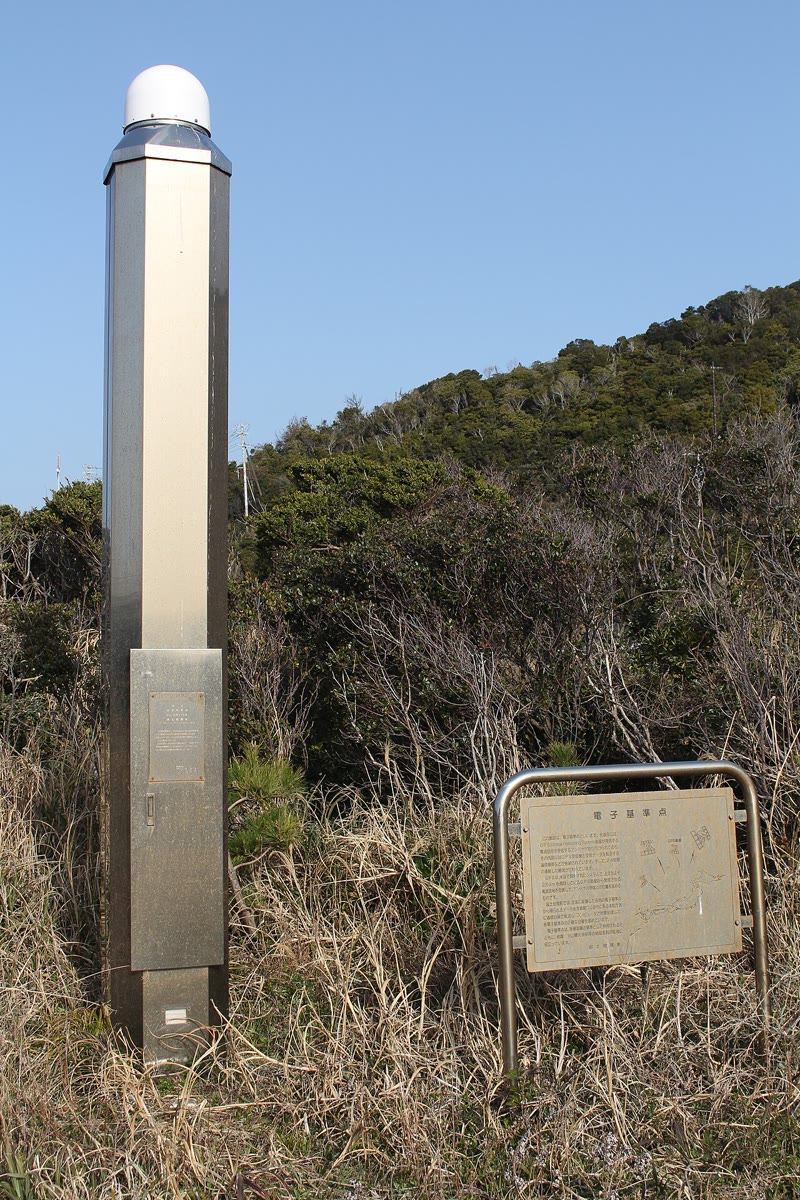
\includegraphics[width=\linewidth]{images/book3/b1-gnss-station.jpg}

{\scriptsize A permanent station in Japan, its antenna under the dome
(Alpsdake, CC BY-SA 4.0).}
\end{minipage}
\end{inthefield}

The velocities of stations in the interiors of two plates give an \omterm{def:b1:plate-kinematics:euler-pole}{Euler vector}
of their own, independent of the geological record. For Eurasia relative to
North America, such a vector predicts \qty{17.0}{mm.yr^{-1}} in Iceland, about
\qty{8}{\percent} less than the \qty{18.6}{mm.yr^{-1}} averaged over
\qty{3.16}{Myr} (figure above). The chord between Reykjavik and Stavanger, both
on stable parts of their plates, lengthens by \qty{17.5}{mm.yr^{-1}}; the
satellite vector predicts \qty{17.1}{mm.yr^{-1}}, the geological one
\qty{18.6}{mm.yr^{-1}}. Across the North Atlantic, a rate measured over a few
decades and a rate averaged over three million years thus agree to within a
tenth: there, the plates move today nearly as they have moved for millions of
years.
% ledger: morvel:gps-eu-na, morvel:eu-na, ngl:reyk, ngl:stas (chord rates computed in calc/ch12.py)

Inside the boundary zone the picture is less simple, for the stations move with
more than the plates. More than a tenth of Iceland lies under ice caps, and
most of them have been losing mass since about 1890: the \omterm{def:b1:layered-earth:layers}{crust} beneath rises as
the load decreases, and moves horizontally away from the thinning ice. The
station at H\"ofn, on the south-east coast near the largest ice cap, rises by
\qty{12.9}{mm.yr^{-1}}.
% ledger: spaans:iceland-gia, ngl:hofn

\section{Exercises}

Take $R = \qty{6371}{km}$ throughout.

\begin{exercise}[$\star$]\label{exo:b1:plate-kinematics:1}
The \omterm{def:b1:plate-kinematics:euler-pole}{Euler vector} of Eurasia relative to North America has the rate
\qty{0.210}{\degree\per\Myr}. (a) Convert it to \unit{rad.yr^{-1}} and to
\unit{rad.s^{-1}}. (b) How long would a full turn take? (c) Compute $\omega R$ in
\unit{mm.yr^{-1}}.
% ledger: morvel:eu-na
\end{exercise}

\begin{exercise}[$\star$]\label{exo:b1:plate-kinematics:2}
With the same \omterm{def:b1:plate-kinematics:euler-pole}{Euler vector}, compute the relative speed of the two plates at
\ang{30}, \ang{60} and \ang{90} from the \omterm{def:b1:plate-kinematics:euler-pole}{Euler pole}. Where along the plate
boundary would the spreading be fastest?
\end{exercise}

\begin{exercise}[$\star$]\label{exo:b1:plate-kinematics:3}
The Jaramillo normal subchron lasted from \qty{1.072}{Ma} to \qty{0.988}{Ma}.
(a) How wide is the stripe it makes on each flank of a ridge with a \omterm{def:b1:plate-kinematics:spreading-rate}{half
spreading rate} of \qty{50}{mm.yr^{-1}}? Of \qty{10}{mm.yr^{-1}}? (b) What is the
total width of the stripe of the present normal chron, which began
\qty{0.781}{Ma}, on a ridge with a half rate of \qty{10}{mm.yr^{-1}}?
% ledger: iodp:gpts2004
\end{exercise}

\begin{exercise}[$\star$]\label{exo:b1:plate-kinematics:4}
On a profile across a ridge, the young edge of the anomaly of chron C2An,
\qty{2.581}{Ma} old, lies \qty{66}{km} west of the axis and \qty{64}{km} east of
it. Compute the two \omterm{def:b1:plate-kinematics:spreading-rate}{half spreading rates} and the \omterm{def:b1:plate-kinematics:spreading-rate}{full spreading rate}. Is the
spreading symmetric?
% ledger: iodp:gpts2004
\end{exercise}

\begin{exercise}[$\star\star$]\label{exo:b1:plate-kinematics:5}
A point of the Gakkel Ridge, in the Arctic Ocean, lies at \ang{85}\,N, \ang{0}\,E.
Compute its angular distance from the Eurasia--North America \omterm{def:b1:plate-kinematics:euler-pole}{Euler pole}
(\ang{61.8}\,N, \ang{139.6}\,E, \qty{0.210}{\degree\per\Myr}) and the spreading
rate there. Compare with the measured rates of \qtyrange{11}{12}{mm.yr^{-1}}.
% ledger: morvel:eu-na
\end{exercise}

\begin{exercise}[$\star\star$]\label{exo:b1:plate-kinematics:6}
At the Azores \omterm{def:b1:plate-kinematics:triple-junction}{triple junction}, \ang{39.44}\,N, \ang{29.83}\,W, compute (a) the
angular distance to the Eurasia--North America \omterm{def:b1:plate-kinematics:euler-pole}{Euler pole}, (b) the spreading
rate, and (c) the \omterm{def:b1:spherical-astronomy:horizontal}{azimuth} of the relative motion. (d) What \omterm{def:b1:field-lab-methods-1:trend-plunge}{trend} do you
predict for the transform faults of the ridge just north of the junction?
% ledger: morvel:eu-na, morvel:azores
\end{exercise}

\begin{exercise}[$\star\star$]\label{exo:b1:plate-kinematics:7}
(a) Write the \omterm{def:b1:plate-kinematics:euler-pole}{Euler vectors} $\vec\omega_{\mathrm{EU\,NA}}$ (\ang{61.8}\,N,
\ang{139.6}\,E, \qty{0.210}{\degree\per\Myr}) and $\vec\omega_{\mathrm{NB\,NA}}$
(\ang{79.2}\,N, \ang{40.2}\,E, \qty{0.233}{\degree\per\Myr}) in Cartesian
components, in \unit{\degree\per\Myr}. (b) Deduce $\vec\omega_{\mathrm{NB\,EU}}$,
its pole and its rate. (c) Why is this the best way to know the motion of Nubia
relative to Eurasia?
% ledger: morvel:eu-na, morvel:nb-na
\end{exercise}

\begin{exercise}[$\star\star$]\label{exo:b1:plate-kinematics:8}
Let $\vec e_x$ point to \ang{0}\,N, \ang{0}\,E, $\vec e_y$ to \ang{0}\,N,
\ang{90}\,E and $\vec e_z$ to the north pole. With Rodrigues' formula, compute
the image of $\vec e_x$ (a) by the rotation of \ang{90} about $\vec e_z$
followed by the rotation of \ang{90} about $\vec e_x$; (b) by the same two
rotations in the opposite order. (c) What does this mean for the
reconstruction of a plate's past positions?
\end{exercise}

\begin{exercise}[$\star\star$]\label{exo:b1:plate-kinematics:9}
Three plates A, B and C meet at a ridge--ridge--ridge junction. Relative to A,
plate B moves at \qty{30}{mm.yr^{-1}} towards the east and plate C at
\qty{40}{mm.yr^{-1}} towards the south. (a) Draw the velocity triangle.
(b) Compute the speed and \omterm{def:b1:spherical-astronomy:horizontal}{azimuth} of C relative to B. (c) What is the \omterm{def:b1:field-lab-methods-1:trend-plunge}{trend} of
the ridge between B and C if it spreads perpendicular to its axis?
\end{exercise}

\begin{exercise}[$\star\star\star$]\label{exo:b1:plate-kinematics:10}
(a) Show that the trace of the matrix $R$ of a rotation by $\alpha$ about any
axis is $1 + 2\cos\alpha$. (b) The matrix
\[
  R = \begin{pmatrix} 0 & 0 & 1\\ 1 & 0 & 0\\ 0 & 1 & 0\end{pmatrix}
\]
is orthogonal with determinant $1$. Find its axis, as a \omterm{def:b1:spherical-astronomy:geographic}{latitude} and \omterm{def:b1:spherical-astronomy:geographic}{longitude},
and its angle. (c) Check your answer by applying $R$ to $\vec e_x$, $\vec e_y$
and $\vec e_z$.
\end{exercise}

\begin{exercise}[$\star\star\star$]\label{exo:b1:plate-kinematics:11}
Before satellite positioning, \omterm{def:b1:plate-kinematics:euler-pole}{Euler poles} were found from the \omterm{def:b1:field-lab-methods-1:trend-plunge}{trends} of
transform faults. (a) Show that the \omterm{def:b1:plate-kinematics:euler-pole}{Euler pole} lies on the \omterm{def:b1:spherical-astronomy:spherical-triangle}{great circle} through
a point of a transform fault that is perpendicular to the fault there, and that
the pole is therefore along $\vec t_1\times\vec t_2$, where $\vec t_1$ and
$\vec t_2$ are unit vectors along two transform faults of the same boundary.
(b) Transform faults \omterm{def:b1:field-lab-methods-1:trend-plunge}{trend} at \ang{95} near the Azores \omterm{def:b1:plate-kinematics:triple-junction}{triple junction}
(\ang{39.44}\,N, \ang{29.83}\,W) and at \ang{103} in Iceland (\ang{64.5}\,N,
\ang{18}\,W). The horizontal unit vector at \omterm{def:b1:spherical-astronomy:geographic}{latitude} $\varphi$ and \omterm{def:b1:spherical-astronomy:geographic}{longitude}
$\lambda$ pointing towards the \omterm{def:b1:spherical-astronomy:horizontal}{azimuth} $\beta$ is $\sin\beta\,\vec e +
\cos\beta\,\vec n$, with $\vec e = (-\sin\lambda, \cos\lambda, 0)$ and $\vec n =
(-\sin\varphi\cos\lambda, -\sin\varphi\sin\lambda, \cos\varphi)$. Locate the
pole. (c) How well do two transforms determine the pole?
% ledger: morvel:eu-na
\end{exercise}

\begin{exercise}[$\star\star\star$]\label{exo:b1:plate-kinematics:12}
The eastward position of a station, every three months for three years, is
(in millimetres, from $t = 0$):
\begin{center}\small
\begin{tabular}{l*{13}{c}}
\hline
$t$ (yr) & 0 & 0.25 & 0.5 & 0.75 & 1 & 1.25 & 1.5 & 1.75 & 2 & 2.25 & 2.5 & 2.75 & 3\\
$x$ (mm) & 4 & 5 & 6 & 15 & 24 & 25 & 26 & 65 & 74 & 75 & 76 & 85 & 94\\
\hline
\end{tabular}
\end{center}
It is made of a steady motion, a seasonal oscillation and a jump caused by an
earthquake. (a) Compute the velocity from the first and last positions.
(b) Compute the nine differences between positions exactly one year apart, and
their median. (c) Explain why the median of one-year differences is a robust
estimate of the steady velocity, and when it would fail.
\end{exercise}

\section{Problem: Iceland splits}

\begin{problem}[{Weekend problem --- the opening of the North Atlantic across
Iceland, measured three ways}]
\label{pb:b1:plate-kinematics:1}
% values: calc/ch12.py (Part II profile invented for the problem; real Euler
% vectors, chron ages and station velocities)
% ledger: morvel:eu-na, morvel:nb-na, iodp:gpts2004, ngl:reyk, ngl:stas, ngl:hofn
Iceland sits on the Mid-Atlantic Ridge, between the North American plate to the
west and the Eurasian plate to the east. Take $R = \qty{6371}{km}$ and, for
Eurasia relative to North America, the \omterm{def:b1:plate-kinematics:euler-pole}{Euler vector} with its pole at
\ang{61.8}\,N, \ang{139.6}\,E and the rate \qty{0.210}{\degree\per\Myr}.

\medskip
\noindent\textbf{Part I --- The plate vector.}
\begin{enumerate}
  \item Convert the rate to \unit{rad.yr^{-1}} and compute $\omega R$ in
        \unit{mm.yr^{-1}}.
  \item Compute the angular distance $\Delta$ from the pole to the centre of
        Iceland, \ang{64.5}\,N, \ang{18}\,W.
  \item Deduce the \omterm{def:b1:plate-kinematics:spreading-rate}{full spreading rate} across Iceland predicted by the plate
        vector.
  \item Compute the \omterm{def:b1:spherical-astronomy:horizontal}{azimuth} of the pole seen from Iceland, and the \omterm{def:b1:spherical-astronomy:horizontal}{azimuth} of the
        motion of Eurasia relative to North America.
  \item Resolve this velocity into its eastward and northward components.
  \item On the Gakkel Ridge, at \ang{86}\,N, \ang{60}\,E, what rate does the same
        vector give? Why is the boundary there so much slower?
\end{enumerate}

\noindent\textbf{Part II --- The magnetic stripes.}
A ship's magnetic profile across the Reykjanes Ridge, south-west of Iceland near
\ang{63}\,N, \ang{23}\,W, run in the direction of spreading, gives the following
distances from the axis to three chron boundaries (a profile constructed for
this problem):
\begin{center}\small
\begin{tabular}{lccc}
\hline
boundary & age (Ma) & west of the axis (km) & east of the axis (km)\\
\hline
base of C1n & 0.781 & 9.7 & 10.1\\
young edge of C2An & 2.581 & 26.8 & 27.3\\
young edge of C5n & 9.779 & 94 & 97\\
\hline
\end{tabular}
\end{center}
\begin{enumerate}[resume]
  \item From the young edge of C5n, compute the two \omterm{def:b1:plate-kinematics:spreading-rate}{half spreading rates}.
  \item Deduce the \omterm{def:b1:plate-kinematics:spreading-rate}{full spreading rate} since \qty{9.8}{Ma}.
  \item Compute the full rate from the two younger boundaries as well. Do the
        three agree? Describe how they change with the age of the boundary.
  \item Is the spreading symmetric? Does the asymmetry change the full rate?
  \item On the Reykjanes Ridge, the boundaries between stripes are displaced
        away from the axis by \qty{5.0}{km} in all, both flanks together.
        Correct the three full rates. Why did the correction matter most for
        the youngest boundary?
  \item How wide is the stripe of the Jaramillo subchron
        (\qtyrange{1.072}{0.988}{Ma}) on each flank, at the corrected half
        rate? Compare with the displacement of question 11. The Jaramillo
        anomaly is nevertheless clearly recognized on Reykjanes Ridge
        profiles, but is absent from the Gakkel Ridge: what does that suggest?
  \item The plate vector predicts \qty{19.0}{mm.yr^{-1}} at the profile. Compare
        with your corrected rates.
\end{enumerate}

\noindent\textbf{Part III --- The satellites.}
The permanent stations REYK (Reykjavik, \ang{64.139}\,N, \ang{21.955}\,W) and
STAS (Stavanger, \ang{59.018}\,N, \ang{5.599}\,E) lie on the North American and
Eurasian plates. Their measured velocities make the chord between them lengthen
by \qty{17.5}{mm.yr^{-1}}.
\begin{enumerate}[resume]
  \item Compute the angular distance between the two stations, and the length
        of the chord.
  \item How long does the chord take to lengthen by one metre?
  \item The plate vector gives STAS a velocity of \qty{18.9}{mm.yr^{-1}} towards
        \ang{114.8} relative to North America. The \omterm{def:b1:spherical-astronomy:spherical-triangle}{great circle} from REYK
        arrives at STAS heading towards \ang{123.1}. Compute the component of
        the velocity along this direction, then the predicted lengthening of
        the chord, which makes the angle $\Delta/2$ with the horizontal at STAS.
  \item Compare the measured and the predicted lengthening. What might explain
        the difference?
  \item Relative to North America, REYK moves at \qty{1.07}{mm.yr^{-1}} to the
        west and \qty{0.97}{mm.yr^{-1}} to the south, and the station HOFN (H\"ofn,
        south-east Iceland) at \qty{21.12}{mm.yr^{-1}} to the east and
        \qty{6.97}{mm.yr^{-1}} to the south. Compute the speed and \omterm{def:b1:spherical-astronomy:horizontal}{azimuth} of HOFN
        relative to REYK.
  \item Compare with Part I. HOFN also rises by \qty{12.9}{mm.yr^{-1}}. Why are
        stations inside Iceland a poor measure of the plate motion?
\end{enumerate}

\noindent\textbf{Part IV --- Ten million years, and the junction to the south.}
\begin{enumerate}[resume]
  \item Over \qty{10}{Myr}, through what angle does Eurasia turn relative to
        North America about the pole?
  \item How far does a point of Eurasia in the middle of Iceland travel along
        its \omterm{def:b1:spherical-astronomy:spherical-triangle}{small circle} in that time? Compare with the corrected width of the
        \omterm{def:b1:layered-earth:layers}{crust} formed since the young edge of C5n in Part II.
  \item At the Azores \omterm{def:b1:plate-kinematics:triple-junction}{triple junction}, the plate vectors give Eurasia
        \qty{22.9}{mm.yr^{-1}} towards \ang{95.1} and Nubia
        \qty{19.2}{mm.yr^{-1}} towards \ang{103.8}, both relative to North
        America. Compute the velocity of Eurasia relative to Nubia.
  \item Is this junction \omterm{def:b1:plate-kinematics:triple-junction}{stable}? What kind of boundary does the velocity of
        question 22 imply between Eurasia and Nubia?
  \item Gather the opening rates of Parts I, II and III. Which agree, and
        which method measures the motion of the plates over the shortest time?
  \item To the nearest millimetre a year, what \omterm{def:b1:plate-kinematics:spreading-rate}{full spreading rate} across
        Iceland do the plate vector and the corrected magnetic stripes both
        give?
\end{enumerate}
\end{problem}
